\documentclass{standalone}

\usepackage{xcolor}

\definecolor{myblue}{HTML}{377EB8}
\definecolor{myred}{HTML}{E41A1C}
\definecolor{myviolet}{HTML}{984EA3}
\definecolor{myteal}{HTML}{008B8B}

\usepackage{tikz}
\usepackage{pgfplots}
\pgfplotsset{compat=newest}

\usepackage{lmodern}
\SetSymbolFont{letters}{bold}{OML}{cmbr}{bx}{it}
\renewcommand{\familydefault}{\sfdefault}

\usepackage{sansmathfonts}

\begin{document}
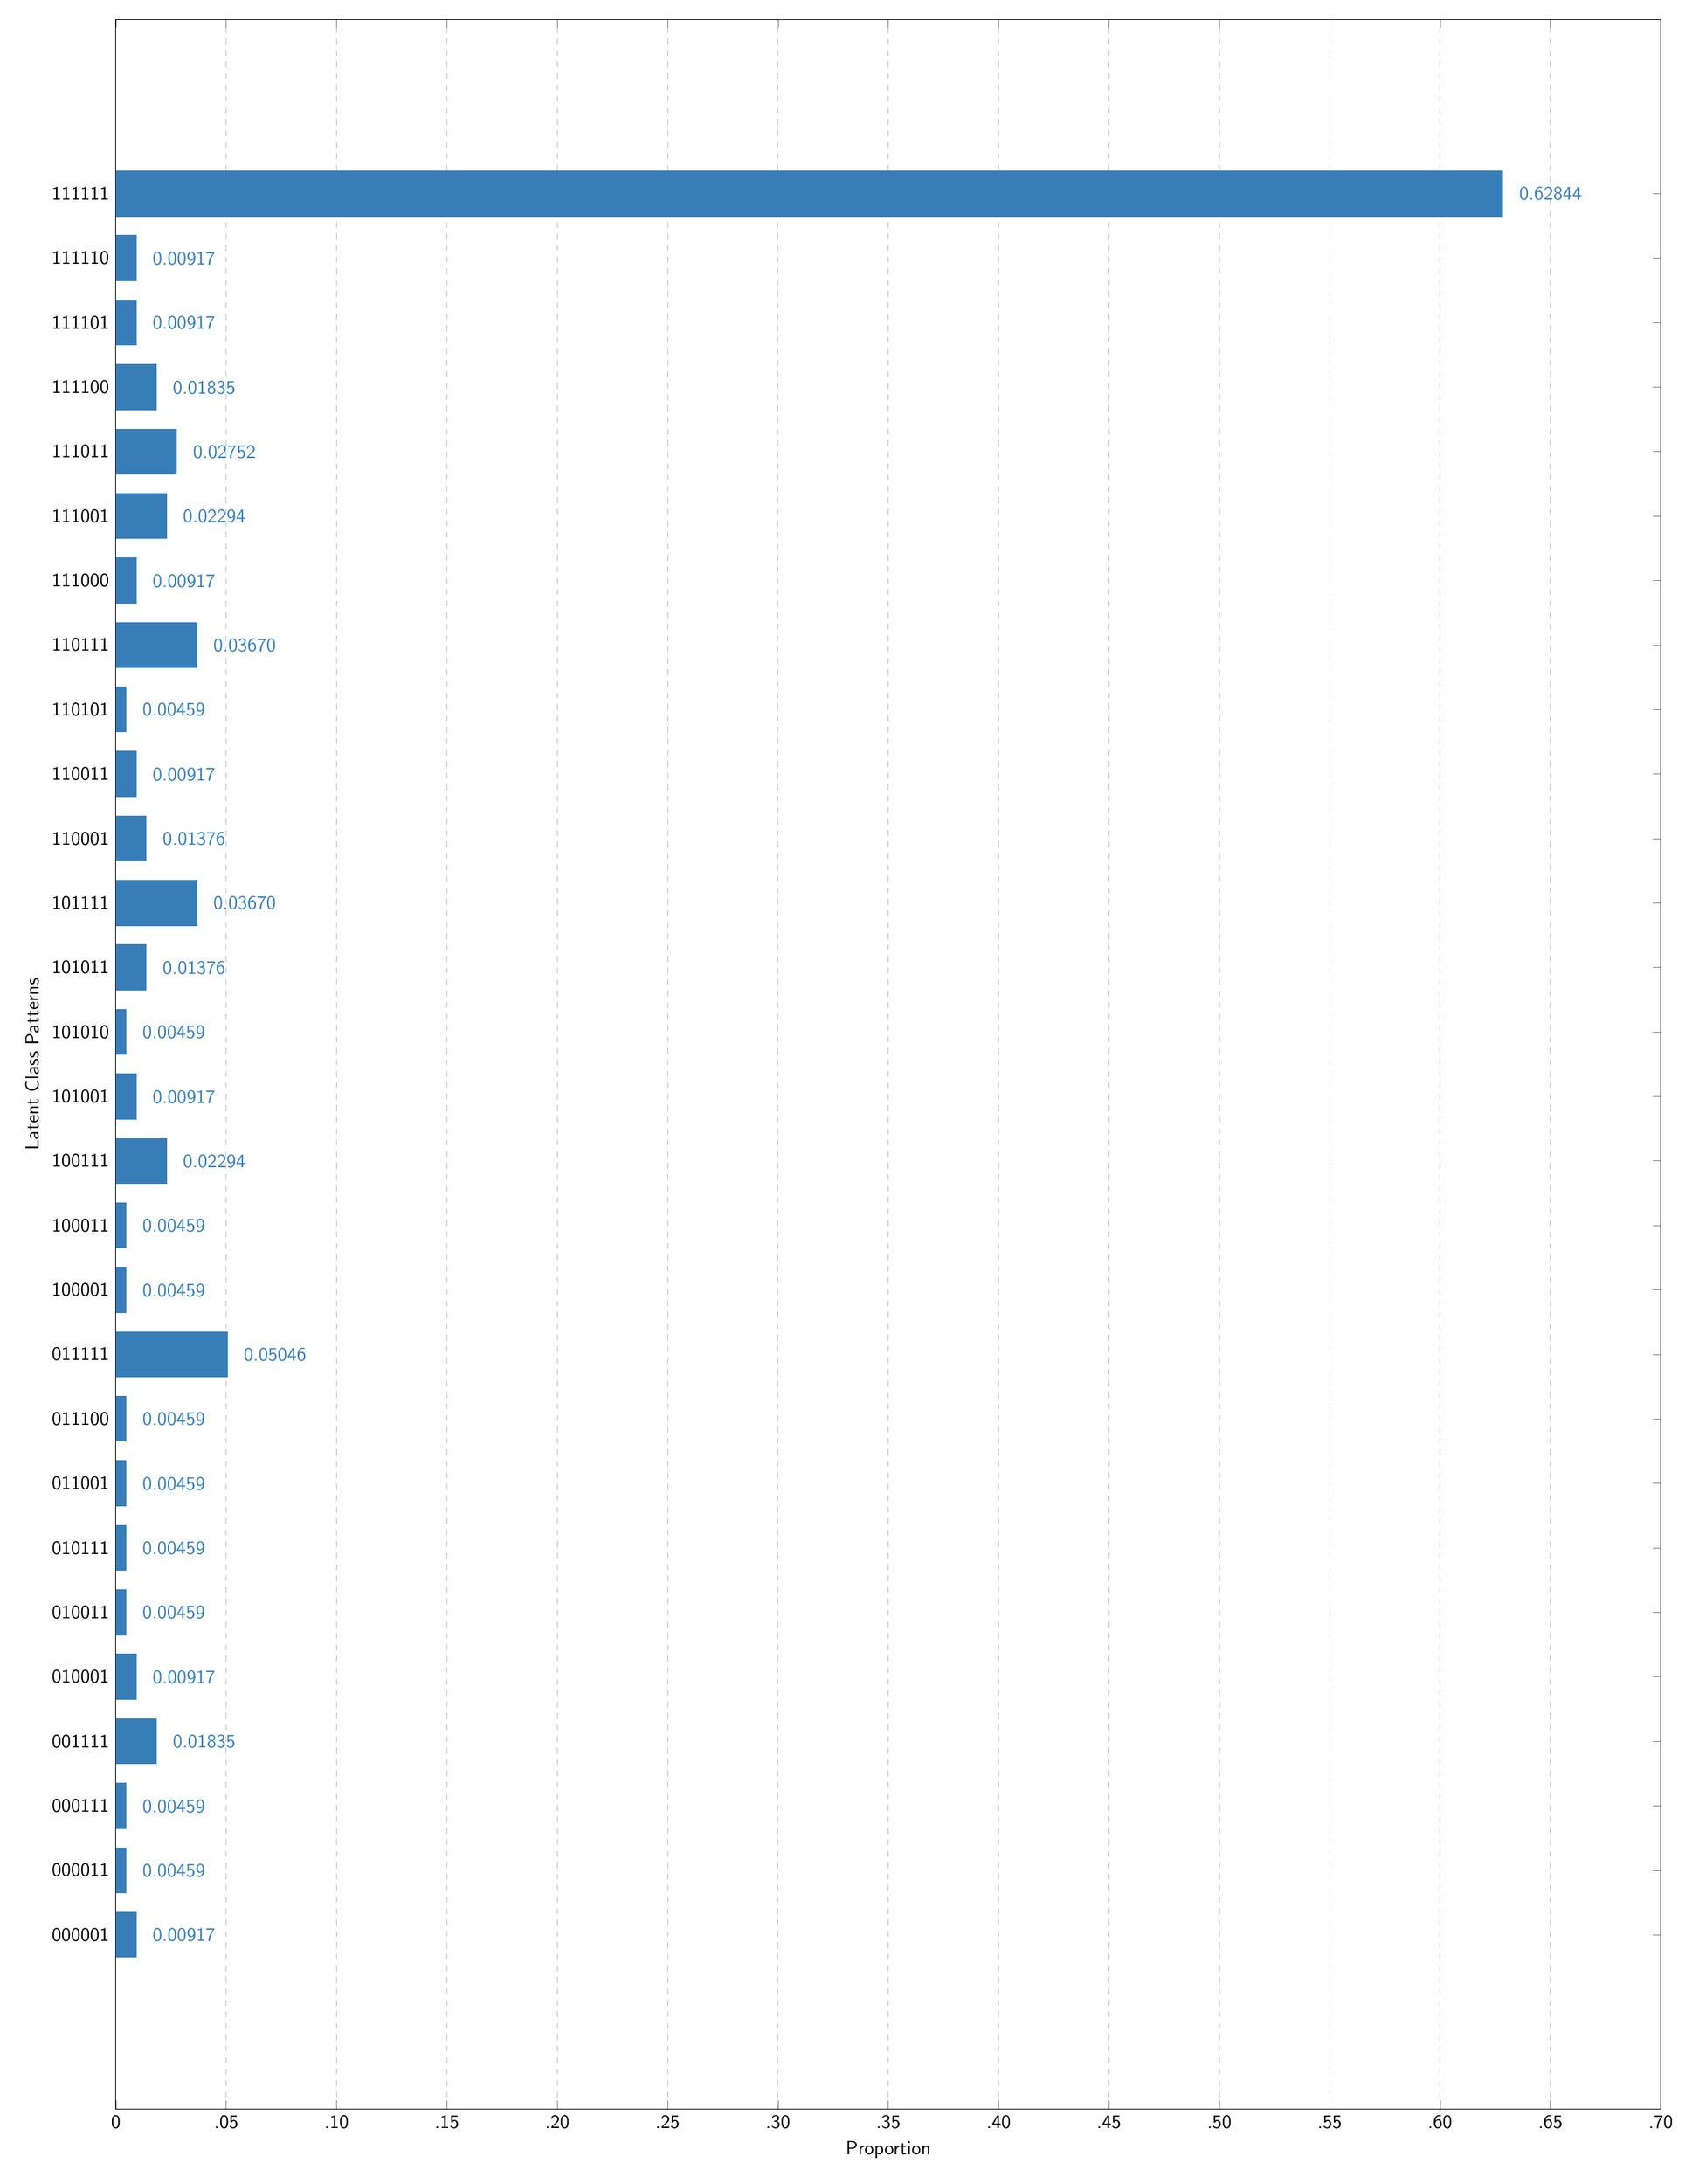
\begin{tikzpicture}
	\begin{axis}[
			xlabel={Proportion},
			ylabel={Latent Class Patterns},
			xmin=0,
			xmax=0.7,
            xtick={
              0,
              .05,
              .10,
              .15,
              .20,
              .25,
              .30,
              .35,
              .40,
              .45,
              .50,
              .55,
              .60,
              .65,
              .70
            },
            xticklabels={
              0,
              .05,
              .10,
              .15,
              .20,
              .25,
              .30,
              .35,
              .40,
              .45,
              .50,
              .55,
              .60,
              .65,
              .70
            },
			ytick={
              1,
              2,
              3,
              4,
              5,
              6,
              7,
              8,
              9,
              10,
              11,
              12,
              13,
              14,
              15,
              16,
              17,
              18,
              19,
              20,
              21,
              22,
              23,
              24,
              25,
              26,
              27,
              28
            },
			yticklabels={
				000001,
				000011,
				000111,
				001111,
				010001,
				010011,
				010111,
				011001,
				011100,
				011111,
				100001,
				100011,
				100111,
				101001,
				101010,
				101011,
				101111,
				110001,
				110011,
				110101,
				110111,
				111000,
				111001,
				111011,
				111100,
				111101,
				111110,
				111111
			},
			width=30cm,
			height=40cm,
			bar width=0.7,
			ymajorgrids=false,
			xmajorgrids=true,
			grid style=dashed,
			nodes near coords,
			nodes near coords align={horizontal},
			every node near coord/.append style={xshift=25pt, yshift=-7pt},
            point meta=explicit symbolic,
		]
		\addplot[myblue, xbar, fill=myblue] coordinates {
			(0.00917,1)[0.00917]
			(0.00459,2)[0.00459]
			(0.00459,3)[0.00459]
			(0.01835,4)[0.01835]
			(0.00917,5)[0.00917]
			(0.00459,6)[0.00459]
			(0.00459,7)[0.00459]
			(0.00459,8)[0.00459]
			(0.00459,9)[0.00459]
			(0.05046,10)[0.05046]
			(0.00459,11)[0.00459]
			(0.00459,12)[0.00459]
			(0.02294,13)[0.02294]
			(0.00917,14)[0.00917]
			(0.00459,15)[0.00459]
			(0.01376,16)[0.01376]
			(0.03670,17)[0.03670]
			(0.01376,18)[0.01376]
			(0.00917,19)[0.00917]
			(0.00459,20)[0.00459]
			(0.03670,21)[0.03670]
			(0.00917,22)[0.00917]
			(0.02294,23)[0.02294]
			(0.02752,24)[0.02752]
			(0.01835,25)[0.01835]
			(0.00917,26)[0.00917]
			(0.00917,27)[0.00917]
			(0.62844,28)[0.62844]
		};
	\end{axis}
\end{tikzpicture}
\end{document}
